\newpage

\section{Metodologi Penelitian}
% Jelaskan metodologi penelitian akan menggunakan diagram, isi diagramnya sesuai dengan alur crisp dm 


Metodologi penelitian yang akan digunakan dalam proyek ini adalah Cross Industry Standard Process for Data Mining (CRISP-DM). CRISP-DM adalah sebuah model proses yang terstruktur dan berulang yang terdiri dari enam fase utama, yaitu Business Understanding, Data Understanding, Data Preparation, Modeling, Evaluation, dan Deployment. Setiap fase memiliki tujuan dan aktivitas spesifik yang membantu dalam mengelola project ini secara efektif. Gambar \ref{fig:crisp-dm} menunjukkan diagram alur metodologi yang berlandaskan prinsip CRISP-DM yang akan diikuti dalam penelitian ini.

\begin{figure}[H]
    \centering
    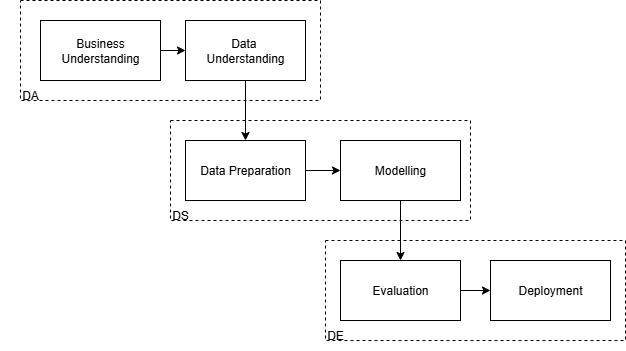
\includegraphics[width=0.7\textwidth]{gambar/diagram.png}
    \caption{Diagram Alur Metodologi}
    \label{fig:crisp-dm}
\end{figure}

% Proyek ini menggunakan metodologi CRISP-DM, yaitu pendekatan bertahap dan berfokus pada kebutuhan bisnis untuk proyek data science.
% 1.	Business Understanding: Memahami tujuan bisnis, lalu ubah menjadi tujuan data science.

% 2.	Data Understanding: Mempelajari data yang tersedia untuk melihat kualitas, pola, dan potensi masalah.

% 3.	Data Preparation: Membersihkan dan siapkan data agar bisa dipakai untuk modeling.

% 4.	Modeling: Membuat dan latih model machine learning untuk menemukan pola dan membuat prediksi.

% 5.	Evaluation: Evaluasi kinerja model dan pastikan hasilnya sesuai kebutuhan bisnis.

% 6.	Deployment: Model yang sudah oke diintegrasikan ke sistem bisnis dan dipantau performanya di dunia nyata.
% penjelasan dari diagram
Setiap fase dalam metodologi CRISP-DM memiliki peran penting dalam memastikan keberhasilan proyek ini. Fase Business Understanding bertujuan untuk memahami konteks bisnis dan mengidentifikasi tujuan yang ingin dicapai melalui analisis data. Fase Data Understanding melibatkan eksplorasi awal terhadap dataset untuk menilai kualitas data, mengidentifikasi pola, dan mendeteksi potensi masalah seperti data yang hilang atau outlier.

Fase Data Preparation fokus pada pembersihan dan transformasi data agar siap digunakan dalam proses pemodelan. Ini termasuk penanganan data yang hilang, normalisasi, dan encoding variabel kategorikal. Fase Modeling adalah tahap di mana berbagai algoritma machine learning diterapkan untuk membangun model prediktif berdasarkan data yang telah dipersiapkan. 

Fase Evaluation melibatkan penilaian kinerja model menggunakan metrik yang relevan untuk memastikan bahwa model memenuhi kebutuhan bisnis yang telah ditetapkan. Terakhir, fase Deployment adalah tahap di mana model yang telah dievaluasi dan disetujui diintegrasikan ke dalam sistem bisnis yang ada, serta dipantau secara berkelanjutan untuk memastikan performa yang optimal di lingkungan nyata.

\subsection{Peran Tim dalam Metodologi}

Data analyst berperan penting dalam setiap fase pertama, mulai dari memahami kebutuhan bisnis, melakukan eksplorasi data, menyiapkan data untuk analisis, membangun dan mengevaluasi model, hingga memastikan bahwa model yang dihasilkan dapat diimplementasikan secara efektif dalam konteks bisnis.

Data scientist akan lebih fokus pada fase Modeling dan PreProcessing, di mana mereka akan menerapkan teknik machine learning yang lebih kompleks, melakukan tuning hyperparameter, serta mengevaluasi model dengan metrik yang lebih mendalam untuk memastikan bahwa model tidak hanya akurat tetapi juga dapat diinterpretasikan dan diandalkan.

Data engineer akan berperan utama dalam fase Deployment, di mana mereka akan memastikan bahwa model yang telah dikembangkan dapat diintegrasikan dengan lancar ke dalam infrastruktur teknologi yang ada. Mereka juga akan bertanggung jawab untuk membangun pipeline data yang efisien, mengelola penyimpanan data, serta memastikan bahwa sistem dapat menangani beban kerja yang diperlukan untuk menjalankan model secara real-time atau batch processing sesuai kebutuhan bisnis.

\subsection{TimeLine Project}
Berikut adalah rincian timeline proyek yang direncanakan untuk setiap fase dalam metodologi CRISP-DM, beserta estimasi waktu yang dibutuhkan untuk menyelesaikan masing-masing fase. Tabel \ref{tb:timeline} merangkum jadwal proyek secara keseluruhan.

\begin{table}[H]
    \centering
    \caption{Timeline Project}
    \label{tb:timeline}
    \begin{tabular}{|l|llllll|}
    \hline
    \rowcolor[HTML]{EFEFEF} 
    \multicolumn{1}{|c|}{\cellcolor[HTML]{EFEFEF}}                                   & \multicolumn{1}{c|}{\cellcolor[HTML]{EFEFEF}Aug} & \multicolumn{4}{c|}{\cellcolor[HTML]{EFEFEF}September}                                                                                                                                                & \multicolumn{1}{c|}{\cellcolor[HTML]{EFEFEF}Oct} \\ \cline{2-7} 
    \rowcolor[HTML]{EFEFEF} 
    \multicolumn{1}{|c|}{\multirow{-2}{*}{\cellcolor[HTML]{EFEFEF}Milestone}}        & \multicolumn{1}{c|}{\cellcolor[HTML]{EFEFEF}W4}  & \multicolumn{1}{c|}{\cellcolor[HTML]{EFEFEF}W1} & \multicolumn{1}{c|}{\cellcolor[HTML]{EFEFEF}W2} & \multicolumn{1}{c|}{\cellcolor[HTML]{EFEFEF}W3} & \multicolumn{1}{c|}{\cellcolor[HTML]{EFEFEF}W4} & \multicolumn{1}{c|}{\cellcolor[HTML]{EFEFEF}W1}  \\ \hline
    \begin{tabular}[c]{@{}l@{}}Project Initiation \& \\ Problem Framing\end{tabular} & \multicolumn{2}{l|}{PM \& DA}                                                                      &                                                 &                                                 &                                                 &                                                  \\ \cline{1-3}
    \begin{tabular}[c]{@{}l@{}}Data Acquisition \& \\ Preparation\end{tabular}       & \multicolumn{1}{l|}{}                            & \multicolumn{1}{l|}{DA \& DS}                   &                                                 &                                                 &                                                 &                                                  \\ \cline{1-1} \cline{3-4}
    \begin{tabular}[c]{@{}l@{}}Model Development \\ \& Experimentation\end{tabular}  &                                                  & \multicolumn{1}{l|}{}                           & \multicolumn{1}{l|}{DA \& DS}                   &                                                 &                                                 &                                                  \\ \cline{1-1} \cline{4-5}
    \begin{tabular}[c]{@{}l@{}}Model Evaluation \\ \& Interpretability\end{tabular}  &                                                  &                                                 & \multicolumn{1}{l|}{}                           & \multicolumn{1}{l|}{DS \& BA}                   &                                                 &                                                  \\ \cline{1-1} \cline{5-6}
    \begin{tabular}[c]{@{}l@{}}Deployment \& \\ Business Integration\end{tabular}    &                                                  &                                                 &                                                 & \multicolumn{1}{l|}{}                           & \multicolumn{1}{l|}{DS \& DE}                   &                                                  \\ \cline{1-1} \cline{6-7} 
    Final Presentation                                                               &                                                  &                                                 &                                                 &                                                 & \multicolumn{1}{l|}{}                           & All Role                                         \\ \hline
    \end{tabular}
\end{table}

Agar lebih jelas lagi, berikut adalah penjabaran dari setiap fase beserta estimasi waktu yang dibutuhkan untuk per stage sesuai jadwal yang diberikan Rakamin Academy. Gambar \ref{fig:timeline0} menunjukkan Timeline Stage0 Project secara keseluruhan.

\begin{figure}[H]
    \centering
    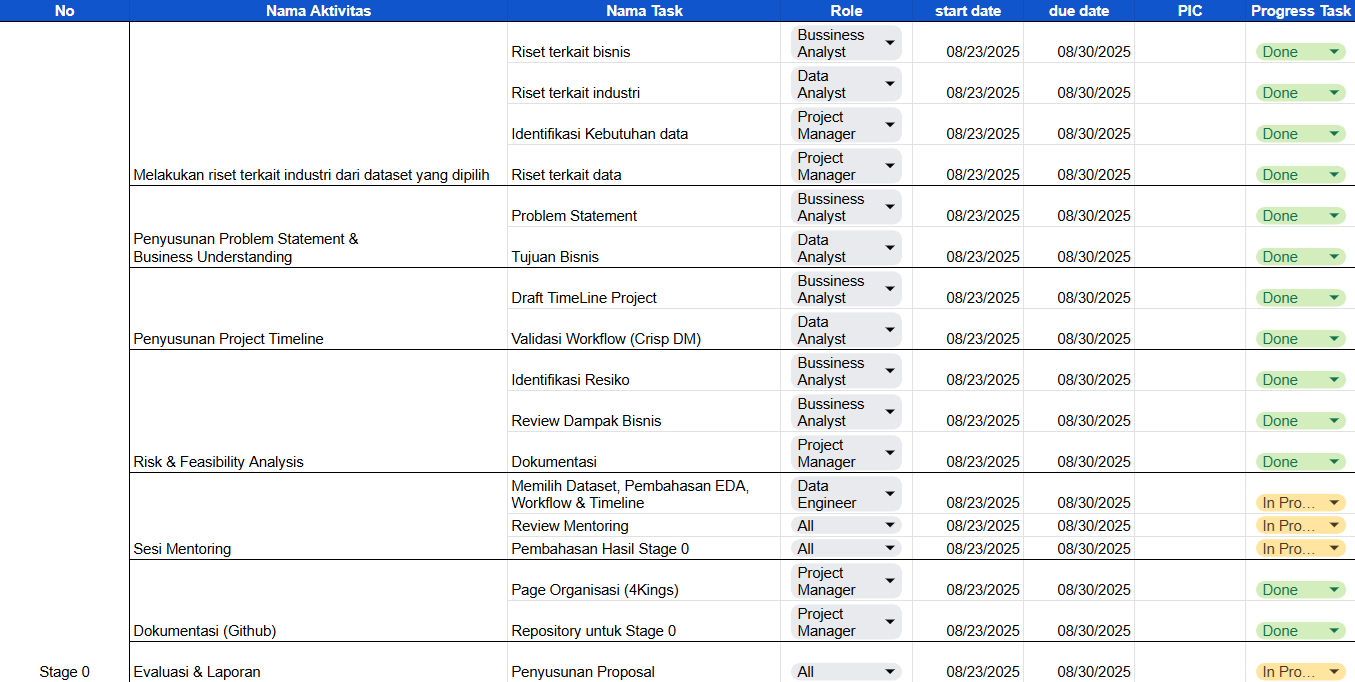
\includegraphics[width=0.9\textwidth]{gambar/timeline0.png}
    \caption{Timeline Stage0 Project}
    \label{fig:timeline0}
\end{figure}

Timeline Stage 0 Project dimulai pada minggu ke-4 bulan Agustus dengan dengan detail seperti pada Gambar \ref{fig:timeline0}. Dibuat juga kolom progress task untuk menandai progress mana yang belum dikerjakan, sedang dikerjakan dan belum mulai dikerjakan. Gambar \ref{fig:timeline1} menunjukkan Timeline Stage1 Project dengan progress task.

\begin{figure}[H]
    \centering
    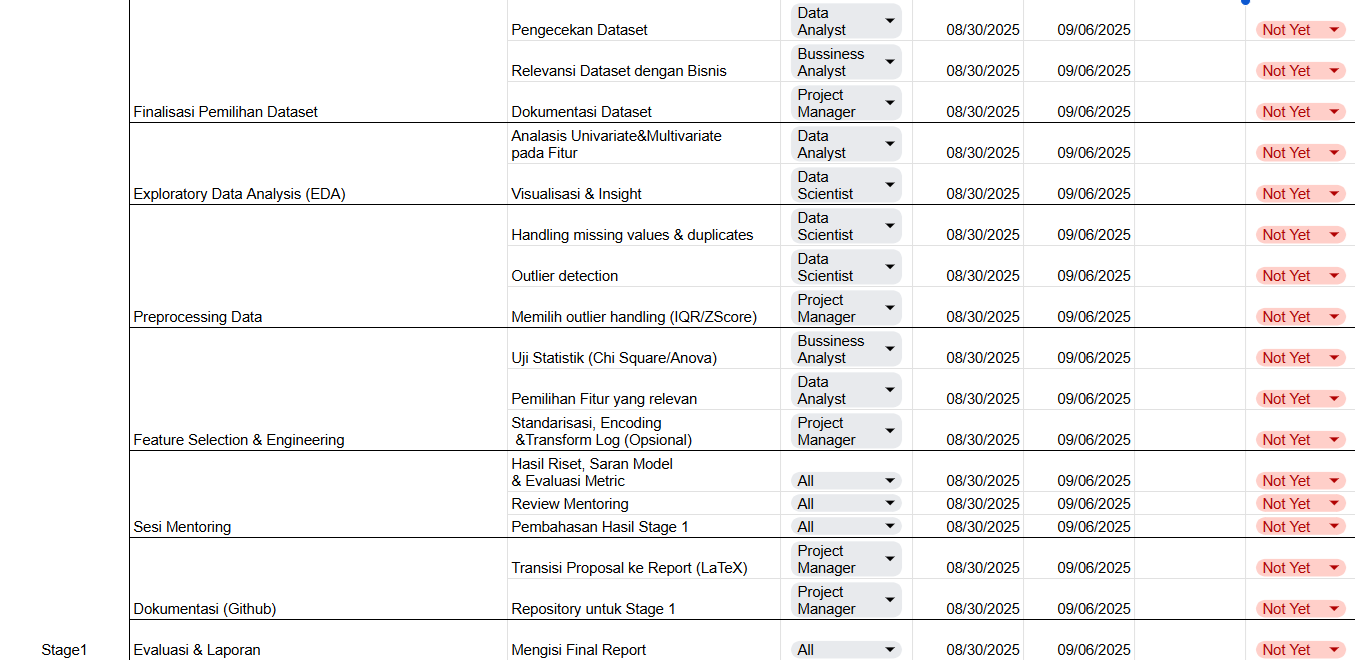
\includegraphics[width=0.9\textwidth]{gambar/timeline1.png}
    \caption{Timeline Stage1 Project dengan Progress Task}
    \label{fig:timeline1}
\end{figure}

Gambar \ref{fig:timeline2} menunjukkan Timeline Stage2 Project dengan progress task.

\begin{figure}[H]
    \centering
    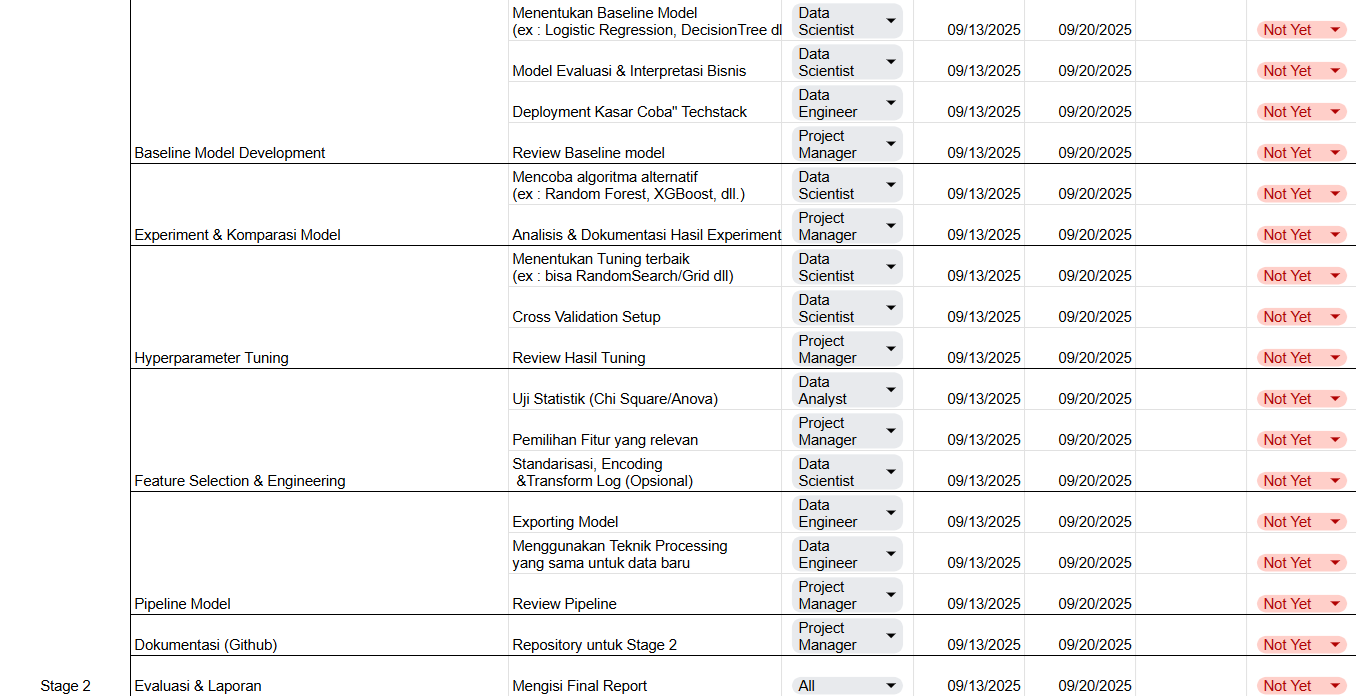
\includegraphics[width=0.9\textwidth]{gambar/timeline2.png}
    \caption{Timeline Stage2 Project dengan Progress Task}
    \label{fig:timeline2}
\end{figure}

Gambar \ref{fig:timeline3} menunjukkan Timeline Stage3 Project dengan progress task.

\begin{figure}[H]
    \centering
    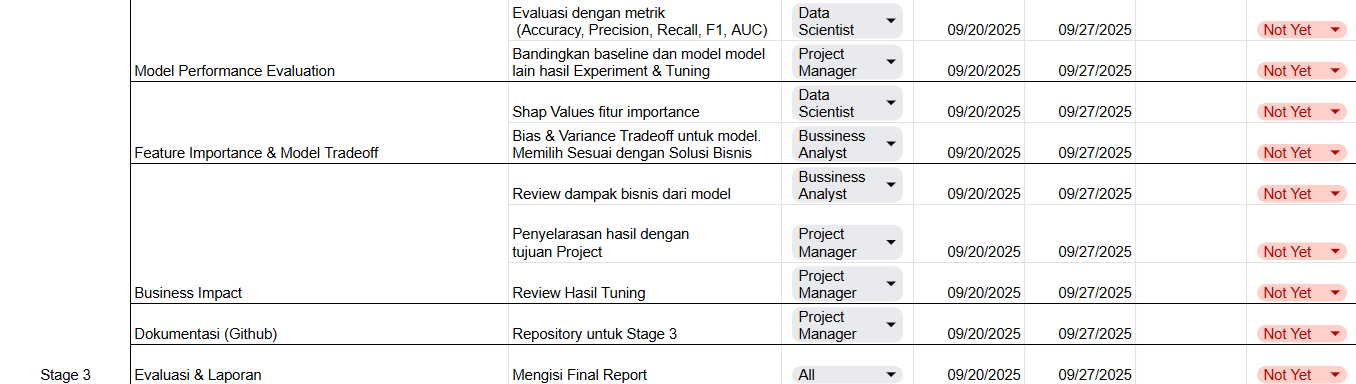
\includegraphics[width=0.9\textwidth]{gambar/timeline3.png}
    \caption{Timeline Stage3 Project dengan Progress Task}
    \label{fig:timeline3}
\end{figure}

Gambar \ref{fig:timeline4} menunjukkan Timeline Stage4 Project dengan progress task.

\begin{figure}[H]
    \centering
    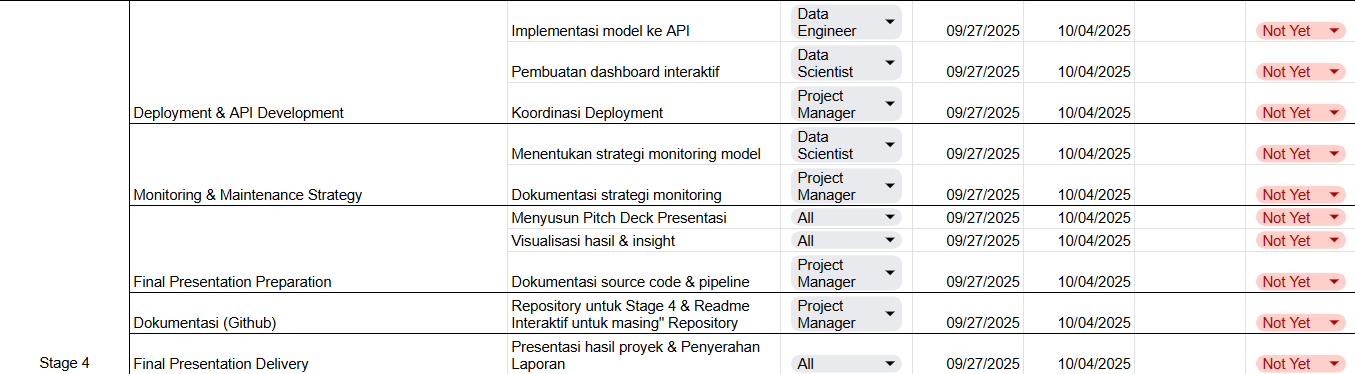
\includegraphics[width=0.9\textwidth]{gambar/timeline4.png}
    \caption{Timeline Stage4 Project dengan Progress Task}
    \label{fig:timeline4}
\end{figure}



\subsection{Risk \& Feasibility Analysis}
Dalam menjalankan proyek ini, terdapat beberapa risiko yang perlu diidentifikasi dan dianalisis untuk memastikan kelancaran proses project. Diharapkan dengan memahami potensi risiko yang ada, tim dapat merancang strategi mitigasi yang efektif guna mengurangi dampak negatif yang mungkin timbul. Tabel \ref{tb:risk-feasibility} merangkum berbagai aspek risiko, potensi risiko yang mungkin dihadapi, strategi mitigasi yang dapat diterapkan, serta penilaian kelayakan dari masing-masing risiko tersebut.



\begin{table}[H]
    \caption{Risk-Feasibility Analysis}
    \label{tb:risk-feasibility}
    \begin{tabular}{|l|l|l|l|}
    \hline
    \rowcolor[HTML]{EFEFEF} 
    \multicolumn{1}{|c|}{\cellcolor[HTML]{EFEFEF}Aspek} & \multicolumn{1}{c|}{\cellcolor[HTML]{EFEFEF}Potensi Risiko}                                                                                                & \multicolumn{1}{c|}{\cellcolor[HTML]{EFEFEF}Strategi Mitigasi}                                                                        & \multicolumn{1}{c|}{\cellcolor[HTML]{EFEFEF}Kelayakan}                                          \\ \hline
    Data                                                & \begin{tabular}[c]{@{}l@{}}Data kandidat bisa \\ tidak lengkap,\\  tidak seimbang \\ (imbalanced), atau\\  mengandung bias \\ (gender, usia).\end{tabular} & \begin{tabular}[c]{@{}l@{}}Lakukan preprocessing, \\ balancing data, feature \\ engineering, serta audit \\ fairness.\end{tabular}    & \begin{tabular}[c]{@{}l@{}}Layak jika dilakukan \\ data cleaning \& \\ monitoring.\end{tabular} \\ \hline
    Teknis                                              & \begin{tabular}[c]{@{}l@{}}Model bisa overfitting\\  atau performa rendah di\\  data baru.\end{tabular}                                                    & \begin{tabular}[c]{@{}l@{}}Gunakan \\ cross-validation, \\ regularisasi, dan \\ retraining berkala.\end{tabular}                      & \begin{tabular}[c]{@{}l@{}}Layak dengan \\ pipeline validasi\\  yang baik.\end{tabular}         \\ \hline
    Operasional                                         & \begin{tabular}[c]{@{}l@{}}HR sulit mengadopsi\\  sistem baru, lebih\\  percaya screening\\  manual.\end{tabular}                                          & \begin{tabular}[c]{@{}l@{}}Berikan pelatihan, buat \\ antarmuka \\ user-friendly, dan \\ jelaskan transparansi \\ model.\end{tabular} & \begin{tabular}[c]{@{}l@{}}Layak jika ada \\ kolaborasi \\ dengan HR.\end{tabular}              \\ \hline
    Etika \& Regulasi                                   & \begin{tabular}[c]{@{}l@{}}Risiko diskriminasi\\  dalam keputusan \\ perekrutan (misalnya \\ gender bias).\end{tabular}                                    & \begin{tabular}[c]{@{}l@{}}Terapkan fairness \\ metrics, hindari variabel \\ sensitif sebagai faktor \\ utama.\end{tabular}           & \begin{tabular}[c]{@{}l@{}}Layak dengan \\ pengawasan \\ etis \& regulasi.\end{tabular}         \\ \hline
    Ekonomi                                             & \begin{tabular}[c]{@{}l@{}}Biaya implementasi dan\\  maintenance model \\ cukup tinggi.\end{tabular}                                                       & \begin{tabular}[c]{@{}l@{}}Bandingkan cost vs \\ benefit (efisiensi waktu, \\ cost per hire, kualitas \\ kandidat).\end{tabular}      & \begin{tabular}[c]{@{}l@{}}Layak jika \\ ROI positif \\ dalam 1–2 tahun.\end{tabular}           \\ \hline
    Keberlanjutan                                       & \begin{tabular}[c]{@{}l@{}}Model bisa usang\\ (model drift) seiring \\ perubahan tren pasar\\  tenaga kerja.\end{tabular}                                  & \begin{tabular}[c]{@{}l@{}}Monitoring performa \\ model, retraining \\ dengan data terbaru \\ setiap periode tertentu.\end{tabular}   & \begin{tabular}[c]{@{}l@{}}Layak dengan \\ komitmen \\ maintenance \\ rutin.\end{tabular}       \\ \hline
    \end{tabular}
    \end{table}

Dengan melakukan analisis risiko ini, tim proyek dapat lebih siap dalam menghadapi tantangan yang mungkin muncul selama pelaksanaan proyek. Setiap risiko yang diidentifikasi telah diberikan strategi mitigasi yang spesifik, sehingga dapat diatasi dengan cara yang paling efektif. Selain itu, penilaian kelayakan dari setiap risiko membantu dalam menentukan prioritas tindakan yang perlu diambil untuk memastikan keberhasilan proyek secara keseluruhan.

\subsection{Penjelasan Dataset}
Dataset yang digunakan dalam proyek ini adalah \texttt{recruitment\_data.csv}, berisi informasi kandidat dan faktor yang dipertimbangkan dalam proses perekrutan. Tujuan pemodelan adalah memprediksi keputusan perekrutan (\textit{HiringDecision}) berdasarkan atribut kandidat.

\subsubsection{Ringkasan Dataset}
\begin{itemize}
    \item \textbf{Jumlah rekaman (baris):} 1{,}500
    \item \textbf{Jumlah fitur (prediktor):} 10
    \item \textbf{Target:} \texttt{HiringDecision} (biner: 0 = tidak diterima, 1 = diterima)
    \item \textbf{Sifat data:} Sintetis (dibuat untuk tujuan pendidikan/proyek data sains)
\end{itemize}

\subsubsection{Definisi Variabel}
Berikut fitur dan target yang tersedia, beserta tipe data, rentang/kategori, dan keterangan singkat. Tabel \ref{tb:var-def} merangkum definisi variabel dalam dataset.

\begin{table}[H]
    \centering
    \caption{Definisi Variabel Dataset}
    \label{tb:var-def}
    \begin{tabular}{|l|l|l|l|}
    \hline
    \rowcolor[HTML]{EFEFEF} 
    Nama Fitur          & Tipe        & Rentang & Keterangan                                                                                      \\ \hline
    Age                 & Numerik     & 20-50   & Umur kandidat                                                                                   \\ \hline
    Gender              & Kategorikal     & 0/1     & 0 = Laki-laki, 1 = Perempuan                                                                    \\ \hline
    EducationLevel      & Kategorikal & 1/2/3/4 & \begin{tabular}[c]{@{}l@{}}1 = S1 (Tipe 1), 2 = S1 (Tipe 2),\\  3 = S2, 4 = S3/PhD\end{tabular} \\ \hline
    ExperienceYears     & Numerik     & 0-15    & Lama pengalaman kerja (tahun)                                                                   \\ \hline
    PreviousCompanies   & Numerik     & 1-5     & \begin{tabular}[c]{@{}l@{}}Jumlah perusahaan tempat bekerja\\  sebelumnya\end{tabular}          \\ \hline
    DistanceFromCompany & Numerik     & 1-50    & Jarak dari rumah ke perusahaan                                                                  \\ \hline
    InterviewScore      & Numerik     & 0-100   & Skor hasil wawancara                                                                            \\ \hline
    SkillScore          & Numerik     & 0-100   & Skor keterampilan teknis                                                                        \\ \hline
    PersonalityScore    & Numerik     & 0-100   & Skor aspek kepribadian                                                                          \\ \hline
    RecruitmentStrategy & Kategorikal & 1/2/3   & \begin{tabular}[c]{@{}l@{}}1 = Agresif, 2 = Moderat, \\ 3 = Konservatif\end{tabular}            \\ \hline
    HiringDecision      & Target      & 0/1     & \begin{tabular}[c]{@{}l@{}}Target: 0 = tidak diterima,\\  1 = diterima\end{tabular}             \\ \hline
    \end{tabular}
    \end{table}

\subsubsection{Catatan Kodefikasi dan Pra-pemrosesan}
\begin{itemize}
    \item \textbf{Gender}: dikodekan sebagai 0 (Laki-laki) dan 1 (Perempuan).
    \item \textbf{EducationLevel}: ordinal 1--4 dengan pemetaan spesifik (S1 Tipe 1, S1 Tipe 2, S2, S3/PhD). Jika korelasi kuat, dapat di \textit{one-hot}.
    \item \textbf{RecruitmentStrategy}: kategorikal 1--3. Umumnya di-\textit{one-hot} untuk model linear; model pohon dapat menggunakan kode numeriknya langsung.
    \item \textbf{Skor (Interview/Skill/Personality)}: berada pada skala 0--100; pertimbangkan penskalaan (\textit{standardization/min-max}) untuk model sensitif skala.
    \item \textbf{Fitur numerik lain} (\texttt{Age}, \texttt{ExperienceYears}, \texttt{PreviousCompanies}, \texttt{DistanceFromCompany}): periksa outlier, distribusi, dan lakukan transformasi/penanganan jika diperlukan.
\end{itemize}

\subsubsection{Sumber dan Lisensi}
Dataset ini dibagikan oleh \textbf{Rabie El Kharoua} dengan lisensi \textbf{CC BY 4.0}. Dataset bersifat \textit{exclusive synthetic} dan ditujukan untuk keperluan edukasi/proyek data sains. Penggunaan diperbolehkan dengan mencantumkan atribusi yang tepat kepada pemilik dataset. DOI dan rincian penyedia data tercantum pada kartu data sumbernya. \parencite{rabie_el_kharoua_2024}

\subsection{EDA (Exploratory Data Analysis)}
EDA adalah langkah awal yang penting dalam analisis data untuk memahami struktur, pola, dan karakteristik dataset. Gambar \ref{fig:eda1} menunjukkan flowchart EDA yang akan dilakukan dalam proyek ini.

\begin{figure}[H]
    \centering
    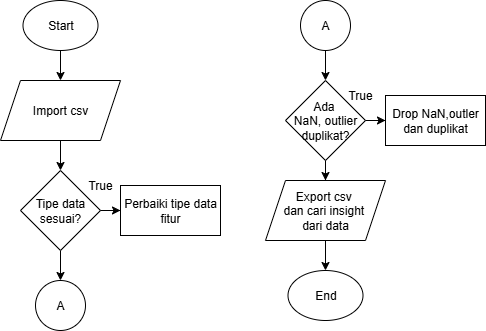
\includegraphics[width=0.6\textwidth]{gambar/flowchartEDA.png}
    \caption{Flowchart EDA}
    \label{fig:eda1}
\end{figure}

Dengan mengikut langkah EDA yang terstruktur, tim dapat memperoleh wawasan yang mendalam tentang dataset, mengidentifikasi potensi masalah, dan menyiapkan data dengan baik untuk tahap pemodelan selanjutnya. EDA membantu memastikan bahwa model yang dibangun didasarkan pada pemahaman yang kuat tentang data, sehingga meningkatkan peluang keberhasilan proyek secara keseluruhan.

\subsubsection{Handle Tipe Data, NaN, \& Duplikasi}
Data wrangling adalah proses penting dalam persiapan data untuk analisis dan pemodelan. Proses ini melibatkan beberapa langkah kunci yang bertujuan untuk membersihkan, mengubah, dan mengorganisir data agar siap digunakan. Dengan menggunakan df.info(), kita dapat memperoleh gambaran umum tentang struktur dataset, termasuk jumlah entri, tipe data setiap kolom, dan informasi tentang nilai yang hilang. Berikut adalah hasil dari df.info() pada dataset yang digunakan dalam proyek ini.

\begin{center}
    \begin{lstlisting}[language=Python, caption=Info Dataset]
        <class 'pandas.core.frame.DataFrame'>
        RangeIndex: 1500 entries, 0 to 1499
        Data columns (total 11 columns):
         #   Column               Non-Null Count  Dtype  
        ---  ------               --------------  -----  
         0   Age                  1500 non-null   int64  
         1   Gender               1500 non-null   int64  
         2   EducationLevel       1500 non-null   int64  
         3   ExperienceYears      1500 non-null   int64  
         4   PreviousCompanies    1500 non-null   int64  
         5   DistanceFromCompany  1500 non-null   float64
         6   InterviewScore       1500 non-null   int64  
         7   SkillScore           1500 non-null   int64  
         8   PersonalityScore     1500 non-null   int64  
         9   RecruitmentStrategy  1500 non-null   int64  
         10  HiringDecision       1500 non-null   int64  
        dtypes: float64(1), int64(10)
        memory usage: 129.0 KB
    \end{lstlisting}
\end{center}

Dari hasil df.info(), kita dapat melihat bahwa dataset terdiri dari 1500 entri dengan 11 kolom. Semua kolom memiliki tipe data numerik (int64 dan float64), dan tidak ada nilai yang hilang (non-null count sama dengan total entries untuk setiap kolom). Ini menunjukkan bahwa dataset sudah cukup bersih dari segi kelengkapan data, namun masih perlu dilakukan pemeriksaan lebih lanjut terhadap distribusi nilai, outlier, dan potensi inkonsistensi lainnya. Walaupun beberapa fitur numerik memiliki makna kategorikal seperti gender, education level, dan recruitment strategy, hal tersebut tidaklah menjadi masalah karena jika dia bertipe object pada akhirnya akan diubah menjadi numerik juga.

Selanjutnya mengecek apakah ada nilai duplikasi pada dataset. Dengan menggunakan df.duplicated().sum(), kita dapat menghitung jumlah baris yang duplikat dalam dataset. Berikut adalah hasil dari pengecekan duplikasi pada dataset yang digunakan dalam proyek ini.

\newpage
\begin{center}
    \begin{lstlisting}[language=Python, caption=Cek Duplikasi Dataset]
        df.duplicated().sum()

        #output
        np.int64(0)
    \end{lstlisting}
\end{center}

Dari hasil pengecekan duplikasi, kita dapat melihat bahwa tidak ada baris yang duplikat dalam dataset (jumlah duplikasi adalah 0). Ini menunjukkan bahwa setiap entri dalam dataset adalah unik, yang merupakan kondisi ideal untuk analisis data dan pemodelan. Dengan tidak adanya duplikasi, kita dapat melanjutkan ke tahap berikutnya dalam proses data wrangling dengan keyakinan bahwa data yang kita miliki sudah bersih dari masalah duplikasi.

\subsubsection{Analisis Fitur Numerik}
Fitur numerik dalam dataset ini meliputi \texttt{Age}, \texttt{ExperienceYears}, \texttt{PreviousCompanies}, \texttt{DistanceFromCompany}, \texttt{InterviewScore}, \texttt{SkillScore}, dan \texttt{PersonalityScore}. Untuk memahami karakteristik dari fitur-fitur ini, kita dapat melakukan analisis statistik deskriptif dan visualisasi distribusi data. Tabel \ref{tb:statistik-deskriptif} merangkum statistik deskriptif dari fitur numerik dalam dataset.

% Age	Gender	EducationLevel	ExperienceYears	PreviousCompanies	DistanceFromCompany	InterviewScore	SkillScore	PersonalityScore	RecruitmentStrategy	HiringDecision
% count	1500.000000	1500.000000	1500.000000	1500.000000	1500.00000	1500.000000	1500.000000	1500.000000	1500.000000	1500.000000	1500.000000
% mean	35.148667	0.492000	2.188000	7.694000	3.00200	25.505379	50.564000	51.116000	49.387333	1.893333	0.310000
% std	9.252728	0.500103	0.862449	4.641414	1.41067	14.567151	28.626215	29.353563	29.353201	0.689642	0.462647
% min	20.000000	0.000000	1.000000	0.000000	1.00000	1.031376	0.000000	0.000000	0.000000	1.000000	0.000000
% 25%	27.000000	0.000000	2.000000	4.000000	2.00000	12.838851	25.000000	25.750000	23.000000	1.000000	0.000000
% 50%	35.000000	0.000000	2.000000	8.000000	3.00000	25.502239	52.000000	53.000000	49.000000	2.000000	0.000000
% 75%	43.000000	1.000000	3.000000	12.000000	4.00000	37.737996	75.000000	76.000000	76.000000	2.000000	1.000000
% max	50.000000	1.000000	4.000000	15.000000	5.00000	50.992462	100.000000	100.000000	100.000000	3.000000	1.000000


% \begin{table}[H]
%     \centering
%     \caption{Deskripsi Statistik Dataset Kandidat}
%     \begin{tabular}{lcccccccccc}
%     \hline
%     Statistik & Age & Gender & Education & Experience & Prev. Comp & Distance & Interview & Skill & Personality & Recruit. Strategy & Hiring Decision \\
%     \hline
%     count & 1500 & 1500 & 1500 & 1500 & 1500 & 1500 & 1500 & 1500 & 1500 & 1500 & 1500 \\
%     mean  & 35.15 & 0.49 & 2.19 & 7.69 & 3.00 & 25.51 & 50.56 & 51.12 & 49.39 & 1.89 & 0.31 \\
%     std   & 9.25 & 0.50 & 0.86 & 4.64 & 1.41 & 14.57 & 28.63 & 29.35 & 29.35 & 0.69 & 0.46 \\
%     min   & 20.00 & 0.00 & 1.00 & 0.00 & 1.00 & 1.00 & 0.00 & 0.00 & 0.00 & 1.00 & 0.00 \\
%     25\%  & 27.00 & 0.00 & 2.00 & 4.00 & 2.00 & 12.84 & 25.00 & 25.75 & 23.00 & 1.00 & 0.00 \\
%     50\%  & 35.00 & 0.00 & 2.00 & 8.00 & 3.00 & 25.50 & 52.00 & 53.00 & 49.00 & 2.00 & 0.00 \\
%     75\%  & 43.00 & 1.00 & 3.00 & 12.00 & 4.00 & 37.74 & 75.00 & 76.00 & 76.00 & 2.00 & 1.00 \\
%     max   & 50.00 & 1.00 & 4.00 & 15.00 & 5.00 & 50.99 & 100.00 & 100.00 & 100.00 & 3.00 & 1.00 \\
%     \hline
%     \end{tabular}
%     \end{table}
    
% \begin{table}[H]
%     \centering
%     \caption{Deskripsi Statistik Dataset Kandidat}
%     \begin{tabular}{lccccccccccc}
%     \hline
%     Statistik & Age & Gender & Education & Experience & Prev. Comp & Distance & Interview & Skill & Personality & Recruit. Strategy & Hiring Decision \\
%     \hline
%     count & 1500 & 1500 & 1500 & 1500 & 1500 & 1500 & 1500 & 1500 & 1500 & 1500 & 1500 \\
%     mean  & 35.15 & 0.49 & 2.19 & 7.69 & 3.00 & 25.51 & 50.56 & 51.12 & 49.39 & 1.89 & 0.31 \\
%     std   & 9.25 & 0.50 & 0.86 & 4.64 & 1.41 & 14.57 & 28.63 & 29.35 & 29.35 & 0.69 & 0.46 \\
%     min   & 20.00 & 0.00 & 1.00 & 0.00 & 1.00 & 1.00 & 0.00 & 0.00 & 0.00 & 1.00 & 0.00 \\
%     25\%  & 27.00 & 0.00 & 2.00 & 4.00 & 2.00 & 12.84 & 25.00 & 25.75 & 23.00 & 1.00 & 0.00 \\
%     50\%  & 35.00 & 0.00 & 2.00 & 8.00 & 3.00 & 25.50 & 52.00 & 53.00 & 49.00 & 2.00 & 0.00 \\
%     75\%  & 43.00 & 1.00 & 3.00 & 12.00 & 4.00 & 37.74 & 75.00 & 76.00 & 76.00 & 2.00 & 1.00 \\
%     max   & 50.00 & 1.00 & 4.00 & 15.00 & 5.00 & 50.99 & 100.00 & 100.00 & 100.00 & 3.00 & 1.00 \\
%     \hline
%     \end{tabular}
%     \end{table}

\begin{table}[H]
    \centering
    \caption{Statistik Deskriptif Fitur Numerik}
    \label{tb:statistik-deskriptif}
    \begin{tabular}{|l|l|l|l|l|l|l|l|l|}
    \hline
    \rowcolor[HTML]{EFEFEF} 
    Fitur               & Count & Mean  & Std   & Min   & 25\%  & 50\%  & 75\%  & Max   \\ \hline
    Age                 & 1500  & 35.15 & 9.25  & 20.00 & 27.00 & 35.00 & 43.00 & 50.00 \\ \hline
    ExperienceYears     & 1500  & 7.69  & 4.64  & 0.00  & 4.00  & 8.00  & 12.00 & 15.00 \\ \hline
    PreviousCompanies   & 1500  & 3.00  & 1.41  & 1.00  & 2.00  & 3.00  & 4.00  & 5.00  \\ \hline
    DistanceFromCompany & 1500  & 25.51 & 14.57 & 1.00  & 12.84 & 25.50 & 37.74 & 50.99 \\ \hline
    InterviewScore      & 1500  & 50.56 & 28.63 & 0.00  & 25.00 & 52.00 & 75.00 & 100.00\\ \hline
    SkillScore          & 1500  & 51.12 & 29.35 & 0.00  & 25.75 & 53.00 & 76.00 & 100.00\\ \hline
    PersonalityScore    & 1500  & 49.39 & 29.35 & 0.00   &23.00&49.00&76.00&100.00\\ \hline
    \end{tabular}
\end{table}

Dari tabel statistik deskriptif, kita dapat melihat bahwa fitur-fitur numerik memiliki variasi yang cukup besar dalam nilai rata-rata, standar deviasi, dan rentang nilai. Misalnya, \texttt{Age} memiliki rata-rata sekitar 35 tahun dengan rentang dari 20 hingga 50 tahun, sementara \texttt{ExperienceYears} memiliki rata-rata sekitar 7.69 tahun dengan rentang dari 0 hingga 15 tahun. Fitur-fitur seperti \texttt{InterviewScore}, \texttt{SkillScore}, dan \texttt{PersonalityScore} menunjukkan distribusi yang luas dengan nilai minimum 0 dan maksimum 100, yang menunjukkan adanya variasi signifikan dalam penilaian kandidat.

Untuk visualisasi distribusi fitur numerik, kita dapat menggunakan boxplot.boxplot memberikan informasi tentang median, kuartil, dan potensi outlier. Gambar \ref{fig:boxplot} menunjukkan boxplot dari beberapa fitur numerik utama.

\begin{figure}[H]
    \centering
    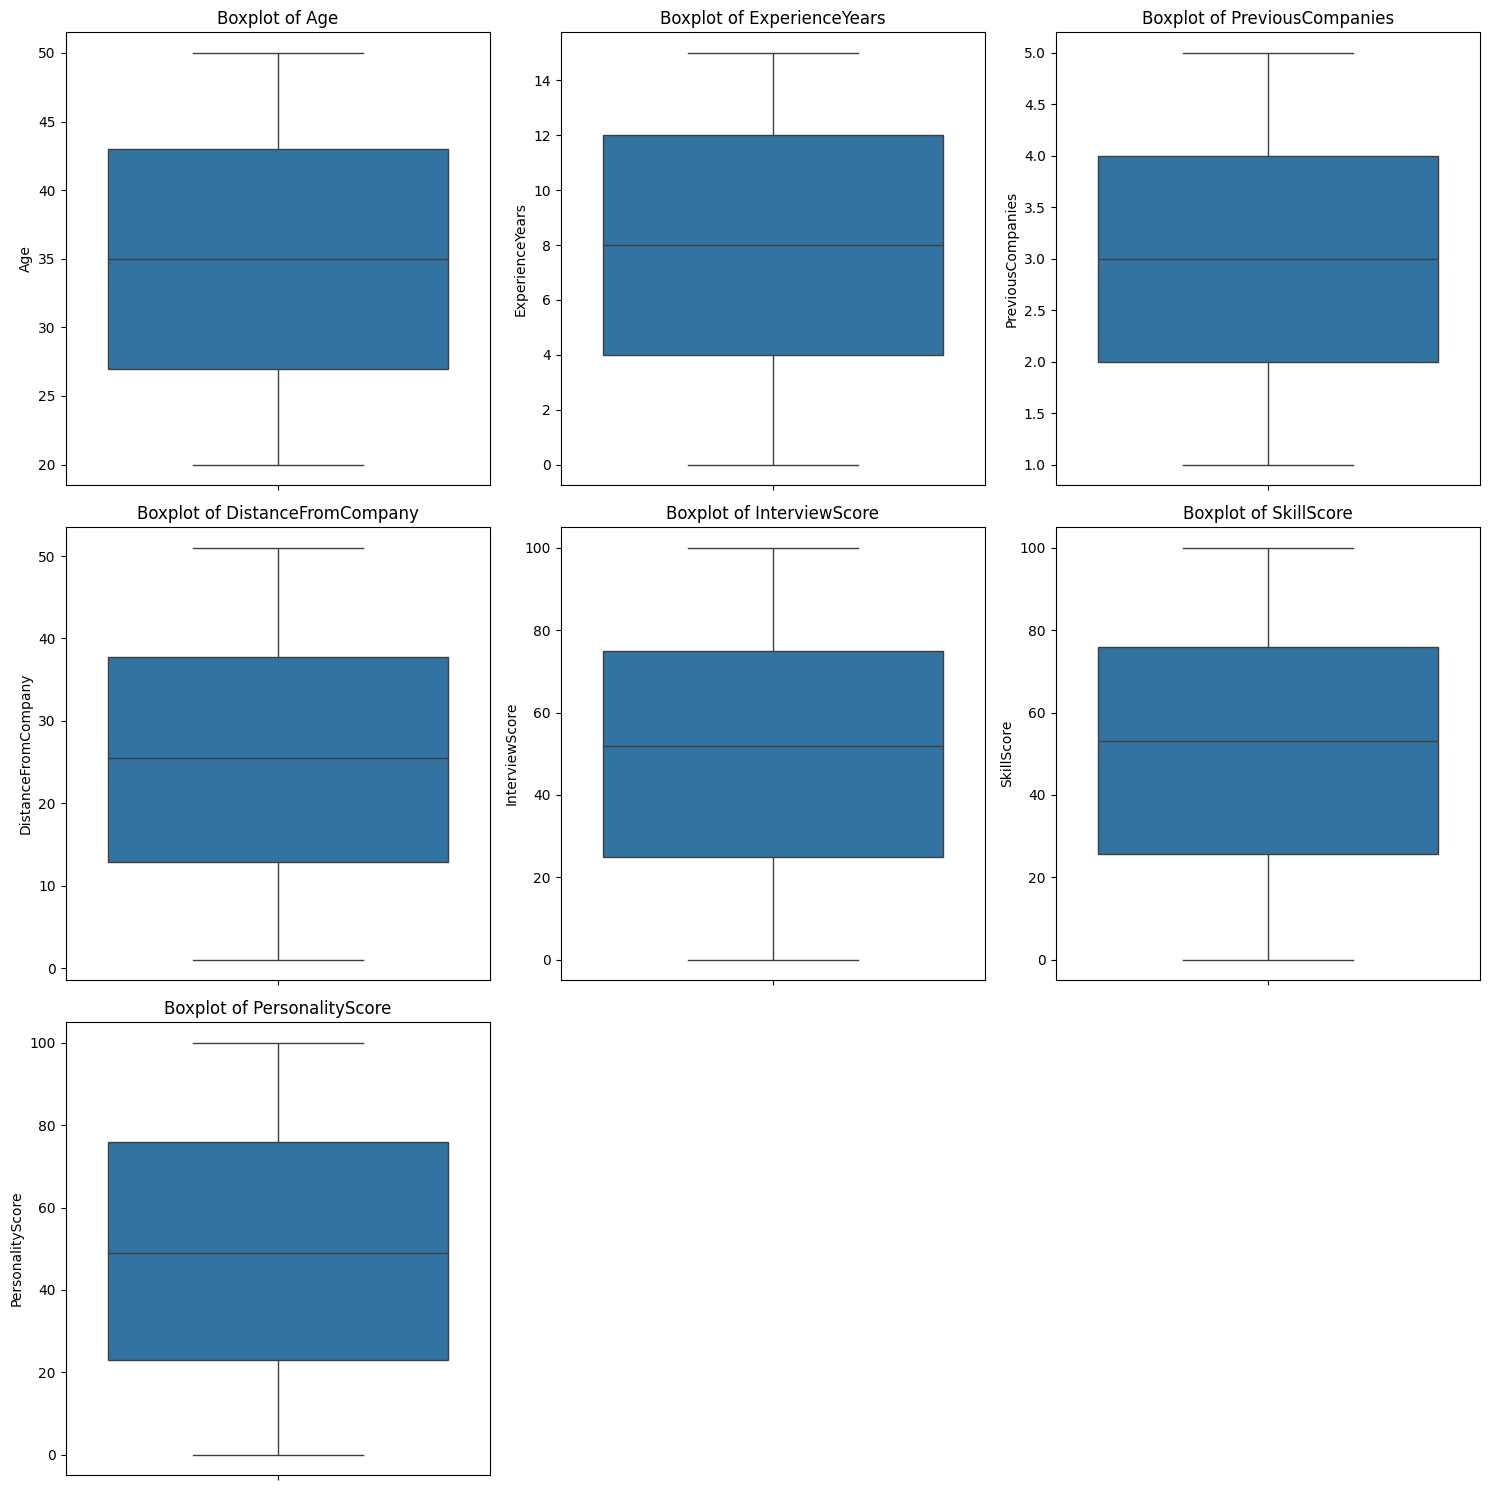
\includegraphics[width=0.8\textwidth]{gambar/boxplot_num.png}
    \caption{Boxplot Fitur Numerik}
    \label{fig:boxplot}
\end{figure}

Dari Gambar \ref{fig:boxplot}, dapat dilihat bahwa semua fitur numerik memiliki tipe distribusi normal serta bersih dari outlier. Hal ini menunjukkan bahwa data sudah cukup baik untuk digunakan dalam pemodelan tanpa perlu penanganan khusus terhadap outlier.

Agar kita lebih memahami hubungan antar fitur numerik, kita dapat menggunakan heatmap untuk memvisualisasikan korelasi antar fitur. Gambar \ref{fig:heatmap} menunjukkan heatmap dari korelasi fitur numerik dalam dataset.

\begin{figure}[H]
    \centering
    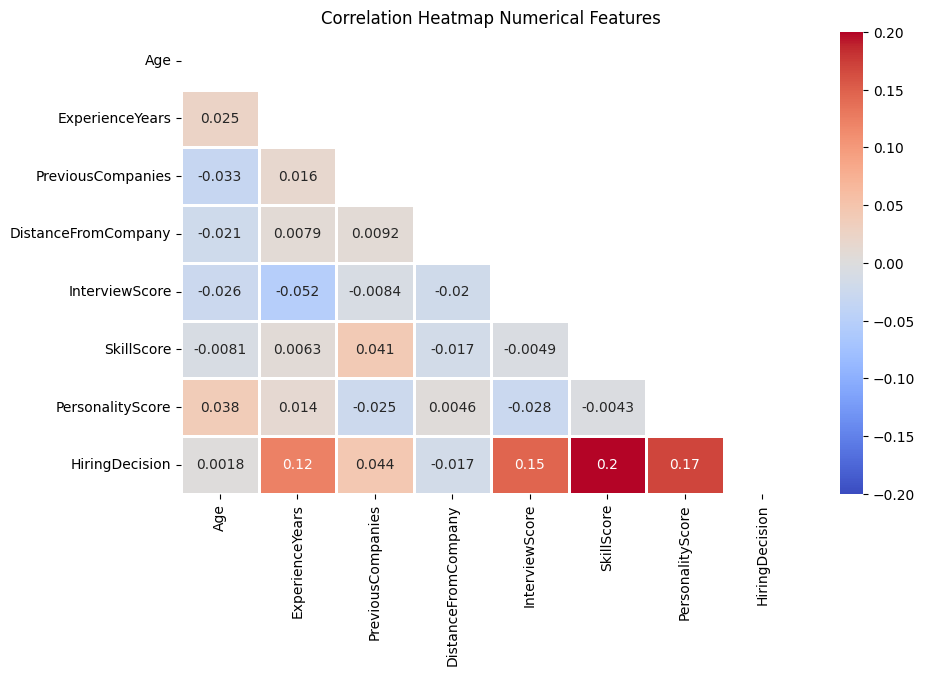
\includegraphics[width=0.8\textwidth]{gambar/heatmap.png}
    \caption{Heatmap Korelasi Fitur Numerik}
    \label{fig:heatmap}
\end{figure}

Dari Gambar \ref{fig:heatmap}, kita dapat melihat bahwa sebagian besar fitur numerik memiliki korelasi yang rendah hingga sedang satu sama lain, dengan nilai korelasi berkisar antara -0.03 hingga 0.2. Tidak ada fitur yang menunjukkan korelasi sangat tinggi (di atas 0.8), yang mengindikasikan bahwa tidak ada multikolinearitas yang signifikan di antara fitur-fitur tersebut. Fitur-fitur seperti \texttt{InterviewScore}, \texttt{SkillScore}, dan \texttt{PersonalityScore} menunjukkan korelasi positif yang signifikan dengan label target (Hiring Decision), yang masuk akal karena ketiga fitur ini berkaitan dengan penilaian kandidat.

Agar memiliki insight yang kuat terhadap data, digunakan juga visualisasi barplot untuk melihat hubungan antara fitur numerik dengan target. Adapun pertanyaan yang dapat dijawab melalui analisis ini antara lain:

\begin{enumerate}
    \item Apakah kandidat yang diterima memiliki usia yang lebih tinggi dibandingkan yang tidak diterima?
    \item Apakah kandidat yang diterima memiliki pengalaman kerja yang lebih banyak dibandingkan yang tidak diterima?
    \item Apakah kandidat yang diterima memiliki riwayat bekerja di lebih banyak perusahaan dibandingkan yang tidak diterima?
    \item Apakah kandidat yang diterima tinggal lebih dekat ke perusahaan dibandingkan yang tidak diterima?
    \item Apakah kandidat yang diterima memiliki Skor Wawancara yang lebih tinggi dibandingkan yang tidak diterima?
    \item Apakah kandidat yang diterima memiliki skor Keterampilan yang lebih tinggi dibandingkan yang tidak diterima?
    \item Apakah kandidat yang diterima memiliki skor Kepribadian yang lebih tinggi dibandingkan yang tidak diterima?
\end{enumerate}

Untuk menjawab pertanyaan-pertanyaan tersebut, kita dapat membuat bar plot dan box plot yang menunjukkan perbandingan rata-rata dari fitur numerik berdasarkan keputusan perekrutan (HiringDecision). Untuk menjawab pertanyaan pertama, kita dapat membuat box plot yang menunjukkan perbandingan rata-rata usia kandidat yang diterima dan tidak diterima. Gambar \ref{fig:usia} menunjukkan box plot dari perbandingan rata-rata usia berdasarkan HiringDecision dalam dataset.

\begin{figure}[H]
    \centering
    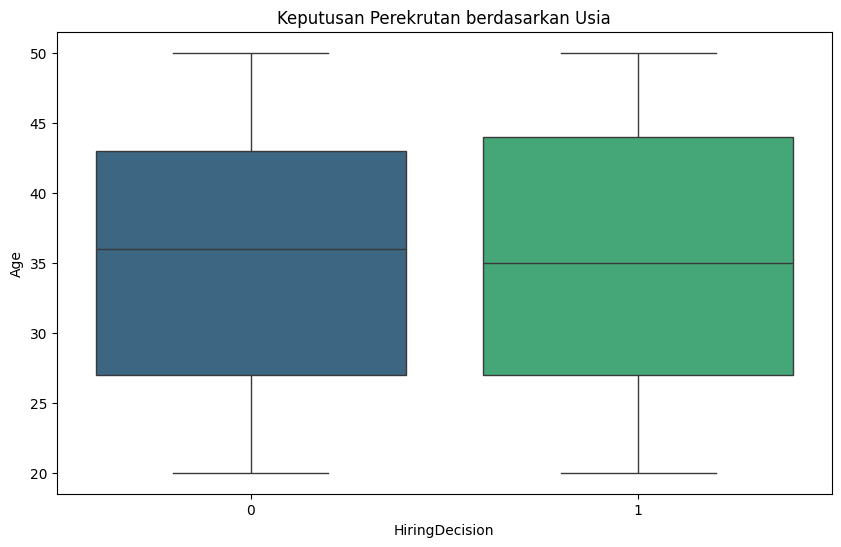
\includegraphics[width=0.6\textwidth]{gambar/usia.png}
    \caption{Box Plot Perbandingan Rata-Rata Usia Berdasarkan HiringDecision}
    \label{fig:usia}
\end{figure}

Dapat dilihat pada Gambar \ref{fig:usia} bahwa tidak ada perbedaan yang signifikan dalam usia antara kandidat yang diterima dan tidak diterima. Rata-rata usia untuk kedua kelompok tersebut tampak cukup mirip, menunjukkan bahwa usia mungkin bukan faktor penentu utama dalam keputusan perekrutan.

Untuk menjawab pertanyaan kedua, kita dapat membuat box plot yang menunjukkan perbandingan rata-rata pengalaman kerja kandidat yang diterima dan tidak diterima. Gambar \ref{fig:exp} menunjukkan box plot dari perbandingan rata-rata pengalaman kerja berdasarkan HiringDecision dalam dataset.

\begin{figure}[H]
    \centering
    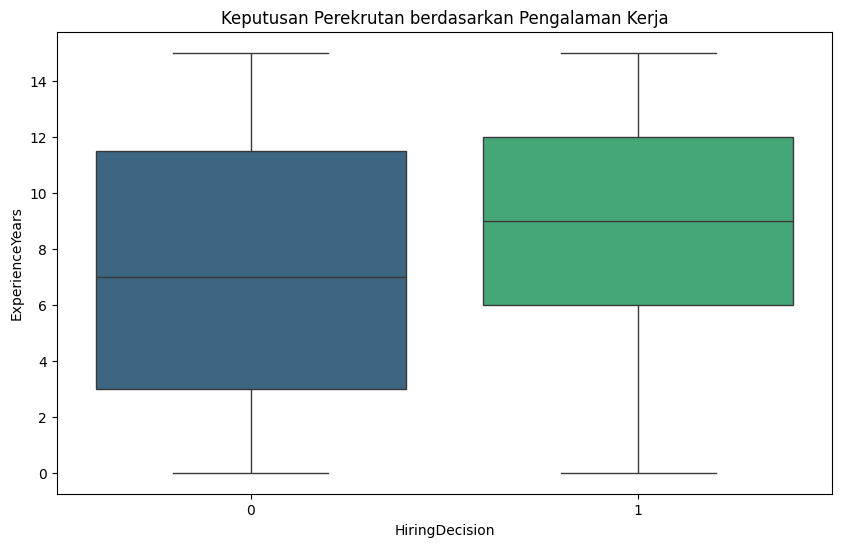
\includegraphics[width=0.6\textwidth]{gambar/exp.png}
    \caption{Box Plot Perbandingan Rata-Rata Pengalaman Kerja Berdasarkan HiringDecision}
    \label{fig:exp}
\end{figure}

Dapat dilihat pada Gambar \ref{fig:exp} bahwa kandidat yang diterima cenderung memiliki pengalaman kerja yang sama dengan kandidat yang tidak diterima. Namun, dapat dilihat bahwa 50\% dari kandidat yang diterima memiliki pengalaman kerja lebih dari 6 tahun yang menandakan bahwa perusahaan cendrung menerima kandidat yang memiliki pengalaman kerja lebih dari besar walaupun hal tersebut bukan menjadi faktor penentu utama dalam keputusan perekrutan karena 50\% dari kandidat yang tidak diterima juga berasal dari rentang pengalaman kerja yang tinggi.

Untuk menjawab pertanyaan ketiga, kita dapat membuat box plot yang menunjukkan perbandingan rata-rata jumlah perusahaan sebelumnya tempat kandidat bekerja berdasarkan HiringDecision. Gambar \ref{fig:prev} menunjukkan box plot dari perbandingan rata-rata jumlah perusahaan sebelumnya berdasarkan HiringDecision dalam dataset.

\begin{figure}[H]
    \centering
    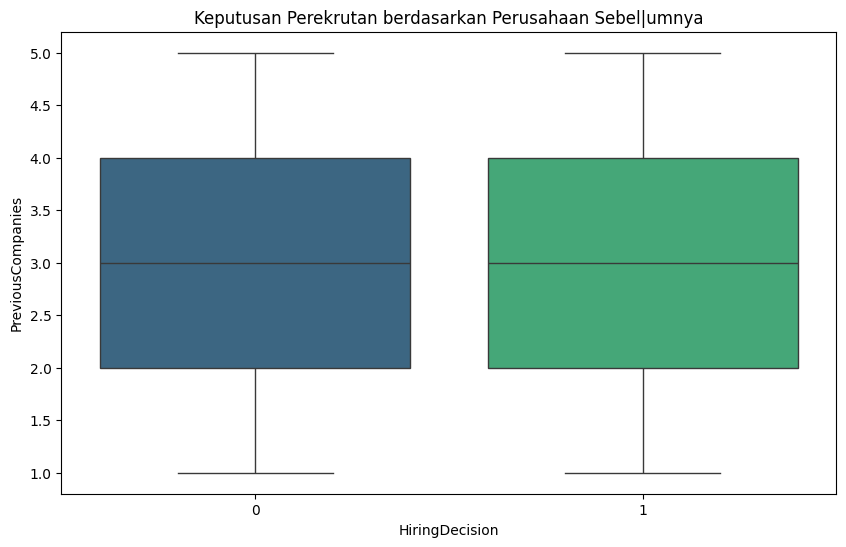
\includegraphics[width=0.6\textwidth]{gambar/prev.png}
    \caption{Box Plot Perbandingan Rata-Rata Jumlah Perusahaan Sebelumnya Berdasarkan HiringDecision}
    \label{fig:prev}
\end{figure}

Dapat dilihat pada Gambar \ref{fig:prev} bahwa tidak ada perbedaan yang signifikan dalam jumlah perusahaan sebelumnya antara kandidat yang diterima dan tidak diterima. Rata-rata jumlah perusahaan sebelumnya untuk kedua kelompok tersebut tampak cukup mirip, menunjukkan bahwa jumlah perusahaan sebelumnya mungkin bukan faktor penentu utama dalam keputusan perekrutan.

Untuk menjawab pertanyaan keempat, kita dapat membuat box plot yang menunjukkan perbandingan rata-rata jarak dari rumah ke perusahaan berdasarkan HiringDecision. Gambar \ref{fig:dist} menunjukkan box plot dari perbandingan rata-rata jarak berdasarkan HiringDecision dalam dataset.

\begin{figure}[H]
    \centering
    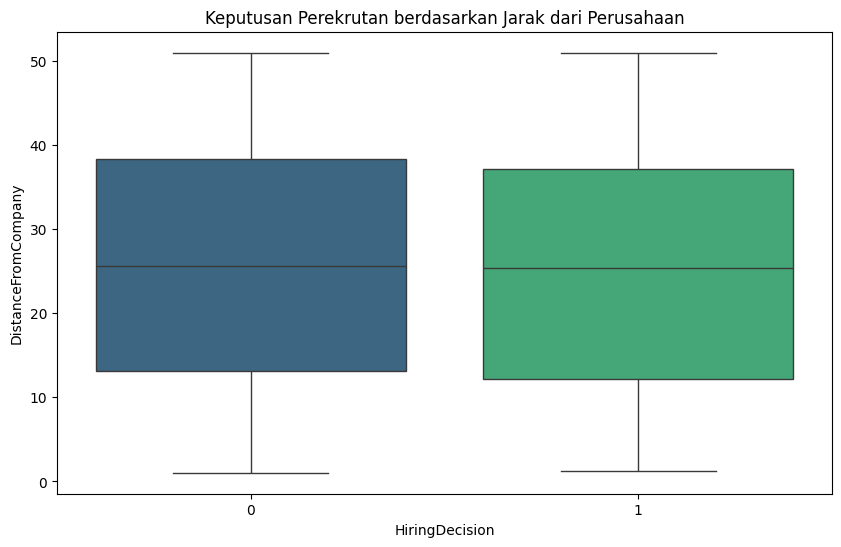
\includegraphics[width=0.6\textwidth]{gambar/dist.png}
    \caption{Box Plot Perbandingan Rata-Rata Jarak dari Rumah ke Perusahaan Berdasarkan HiringDecision}
    \label{fig:dist}
\end{figure}

Dapat dilihat pada Gambar \ref{fig:dist} bahwa tidak ada perbedaan yang signifikan dalam jarak dari rumah ke perusahaan antara kandidat yang diterima dan tidak diterima. Rata-rata jarak untuk kedua kelompok tersebut tampak cukup mirip, menunjukkan bahwa jarak dari rumah ke perusahaan mungkin bukan faktor penentu utama dalam keputusan perekrutan.

Untuk menjawab pertanyaan kelima, kita dapat membuat box plot yang menunjukkan perbandingan rata-rata skor wawancara berdasarkan HiringDecision. Gambar \ref{fig:interview} menunjukkan box plot dari perbandingan rata-rata skor wawancara berdasarkan HiringDecision dalam dataset.

\begin{figure}[H]
    \centering
    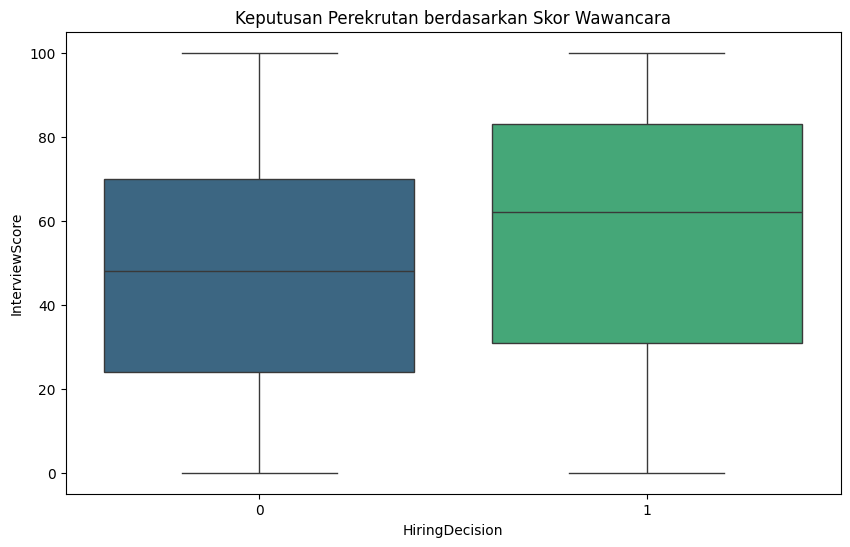
\includegraphics[width=0.6\textwidth]{gambar/interview.png}
    \caption{Box Plot Perbandingan Rata-Rata Skor Wawancara Berdasarkan HiringDecision}
    \label{fig:interview}
\end{figure}

Dapat dilihat pada Gambar \ref{fig:interview} bahwa kandidat yang diterima cenderung memiliki skor wawancara yang lebih tinggi dibandingkan dengan kandidat yang tidak diterima. Rata-rata skor wawancara untuk kandidat yang diterima tampak lebih tinggi, menunjukkan bahwa skor wawancara mungkin menjadi faktor penting dalam keputusan perekrutan.

Untuk menjawab pertanyaan keenam, kita dapat membuat box plot yang menunjukkan perbandingan rata-rata skor keterampilan berdasarkan HiringDecision. Gambar \ref{fig:skill} menunjukkan box plot dari perbandingan rata-rata skor keterampilan berdasarkan HiringDecision dalam dataset.

\begin{figure}[H]
    \centering
    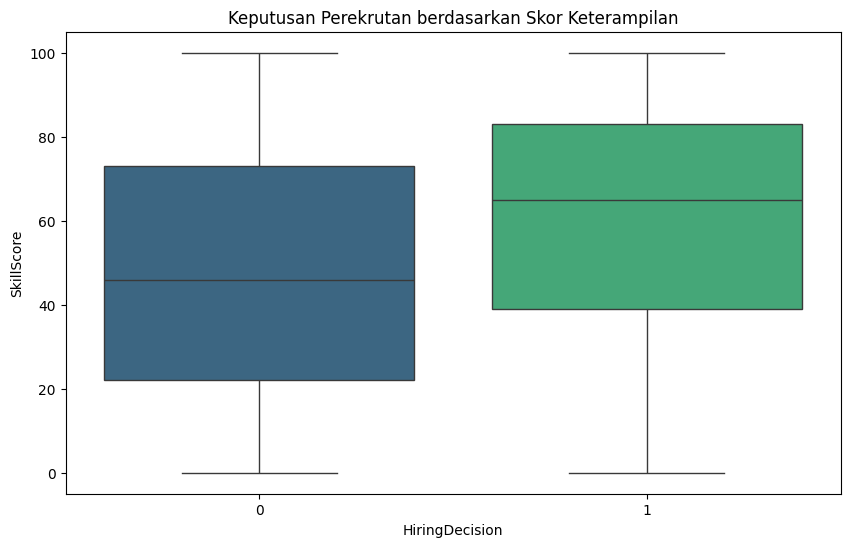
\includegraphics[width=0.6\textwidth]{gambar/skill.png}
    \caption{Box Plot Perbandingan Rata-Rata Skor Keterampilan Berdasarkan HiringDecision}
    \label{fig:skill}
\end{figure}

Dapat dilihat pada Gambar \ref{fig:skill} bahwa kandidat yang diterima cenderung memiliki skor keterampilan yang lebih tinggi dibandingkan dengan kandidat yang tidak diterima. Rata-rata skor keterampilan untuk kandidat yang diterima tampak lebih tinggi, menunjukkan bahwa skor keterampilan mungkin menjadi faktor penting dalam keputusan perekrutan.

Untuk menjawab pertanyaan ketujuh, kita dapat membuat box plot yang menunjukkan perbandingan rata-rata skor kepribadian berdasarkan HiringDecision. Gambar \ref{fig:personality} menunjukkan box plot dari perbandingan rata-rata skor kepribadian berdasarkan HiringDecision dalam dataset.

\begin{figure}[H]
    \centering
    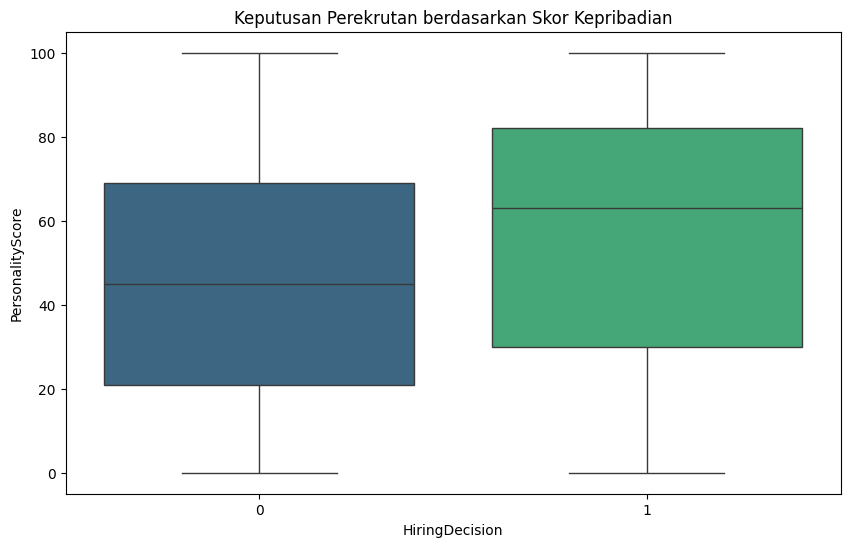
\includegraphics[width=0.6\textwidth]{gambar/personality.png}
    \caption{Box Plot Perbandingan Rata-Rata Skor Kepribadian Berdasarkan HiringDecision}
    \label{fig:personality}
\end{figure}

Dapat dilihat pada Gambar \ref{fig:personality} bahwa kandidat yang diterima cenderung memiliki skor kepribadian yang lebih tinggi dibandingkan dengan kandidat yang tidak diterima. Rata-rata skor kepribadian untuk kandidat yang diterima tampak lebih tinggi, menunjukkan bahwa skor kepribadian mungkin menjadi faktor penting dalam keputusan perekrutan.



Dengan analisa yang dilakukan sebelumnya, kita sudah mengetahui bahwa data sudah bersih dan siap untuk dilakukan pemodelan, kita juga sudah mengetahui fitur-fitur mana saja yang memiliki korelasi yang cukup tinggi dengan target dan mana fitur yang tidak memiliki korelasi sama sekali. Namun uji statistik tetap perlu dilakukan untuk memastikan fitur-fitur yang akan digunakan dalam pemodelan adalah fitur yang benar-benar memiliki korelasi yang signifikan dengan target. Karena label target adalah kategorikal (1/0) dan fitur yang akan diuji adalah numerik, maka uji statistik yang tepat adalah uji t-test. Berikut adalah hasil uji t-test yang dilakukan pada fitur-fitur numerik dalam dataset. Tabel \ref{tb:t-test} merangkum hasil uji t-test untuk setiap fitur numerik.

\begin{table}[H]
    \centering
    \caption{Hasil Uji T-Test Fitur Numerik}
    \label{tb:t-test}
    \begin{tabular}{|l|l|l|l|}
    \hline
    \rowcolor[HTML]{EFEFEF} 
    Fitur               & T-Stat & P-Value & Kesimpulan                                                                                     \\ \hline
    Age                 & 0.0716      & $9.43 \times 10^{-1}$ & Tidak ada perbedaan signifikan (\(p >= 0.05\))                                                     \\ \hline
    ExperienceYears     & 4.7770      & $1.95 \times 10^{-6}$  & Ada perbedaan signifikan (\(p < 0.05\))                                                            \\ \hline
    PreviousCompanies   & 1.7056      & $8.83 \times 10^{-2}$  & Tidak ada perbedaan signifikan (\(p >= 0.05\))                                                     \\ \hline
    DistanceFromCompany & -0.6500     & $5.16 \times 10^{-1}$  & Tidak ada perbedaan signifikan (\(p >= 0.05\))                                                     \\ \hline
    InterviewScore      & 5.7146      & $1.32 \times 10^{-8}$  & Ada perbedaan signifikan (\(p < 0.05\))                                                            \\ \hline
    SkillScore          & 8.0515      & $1.7 \times 10^{-15}$  & Ada perbedaan signifikan (\(p < 0.05\))                                                            \\ \hline
    PersonalityScore    & 6.6436      & $4.27 \times 10^{-11}$  & Ada perbedaan signifikan (\(p < 0.05\))                                                            \\ \hline
    \end{tabular}
\end{table}

Dari tabel hasil uji t-test, kita dapat melihat bahwa fitur-fitur seperti \texttt{ExperienceYears}, \texttt{InterviewScore}, \texttt{SkillScore}, dan \texttt{PersonalityScore} menunjukkan perbedaan yang signifikan antara kelompok kandidat yang diterima dan tidak diterima (HiringDecision) (\(p < 0.05\)). Ini mengindikasikan bahwa fitur-fitur ini memiliki pengaruh yang kuat terhadap keputusan perekrutan dan sebaiknya dipertimbangkan dalam pemodelan. Sebaliknya, fitur seperti \texttt{Age}, \texttt{PreviousCompanies}, dan \texttt{DistanceFromCompany} tidak menunjukkan perbedaan yang signifikan (\(p >= 0.05\)), sehingga mungkin kurang relevan untuk dimasukkan dalam model prediksi.

\subsection{Analisis Fitur Kategorikal}
Fitur kategorikal dalam dataset ini meliputi Gender, EducationLevel, dan RecruitmentStrategy. Untuk memahami karakteristik dari fitur-fitur ini, kita dapat melakukan analisis frekuensi dan visualisasi distribusi data. Adapun beberapa pertanyaan yang dapat dijawab melalui analisis ini antara lain:

\begin{enumerate}
    \item Berapa perbandingan jumlah kandidat yang diterima dan tidak ?
    \item Apakah EducationLevel berperan besar dalam keputusan hiring ?
    \item Berapa perbandingan pria dan wanita yang diterima dan tidak ?
    \item Apakah RecruitmentStrategy berperan besar dalam keputusan hiring ?
\end{enumerate}

Untuk menjawab pertanyaan-pertanyaan tersebut, kita dapat menggunakan visualisasi seperti bar plot. Untuk menjawab pertanyaan pertama, kita dapat membuat bar plot yang menunjukkan jumlah kandidat yang diterima dan tidak diterima. Gambar \ref{fig:barplot1} menunjukkan bar plot dari distribusi HiringDecision dalam dataset.

\begin{figure}[H]
    \centering
    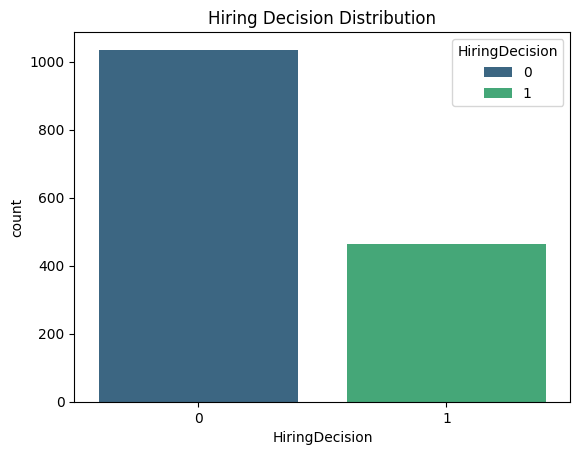
\includegraphics[width=0.6\textwidth]{gambar/barplot1.png}
    \caption{Bar Plot Distribusi HiringDecision}
    \label{fig:barplot1}
\end{figure}

Didapat perbandingnan 31:69, artinya 31\% kandidat diterima dan 69\% tidak diterima. Hal ini menunjukkan bahwa proses perekrutan cukup selektif, dengan hanya sekitar sepertiga dari total kandidat yang berhasil diterima. Informasi ini penting untuk memahami tingkat persaingan di antara kandidat dan dapat membantu dalam merancang strategi perekrutan yang lebih efektif.

% Untuk menjawab pertanyaan kedua, kita dapat membuat bar plot yang menunjukkan hubungan antara InterviewScore dan HiringDecision. Gambar \ref{fig:barplot2} menunjukkan bar plot dari distribusi InterviewScore berdasarkan HiringDecision.

% \begin{figure}[H]
%     \centering
%     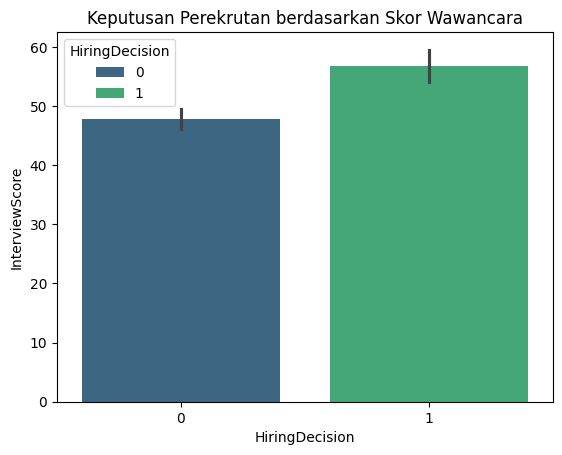
\includegraphics[width=0.6\textwidth]{gambar/barplot2.png}
%     \caption{Bar Plot InterviewScore vs HiringDecision}
%     \label{fig:barplot2}
% \end{figure}

% Dari Gambar \ref{fig:barplot2}, kita dapat melihat bahwa kandidat dengan InterviewScore yang lebih tinggi cenderung memiliki peluang lebih besar untuk diterima (HiringDecision = 1). Hal ini menunjukkan bahwa skor wawancara merupakan faktor penting dalam keputusan perekrutan, dan kandidat yang tampil baik dalam wawancara memiliki peluang lebih besar untuk berhasil dalam proses seleksi.

Untuk menjawab pertanyaan kedua, kita dapat membuat bar plot yang menunjukkan hubungan antara EducationLevel dan HiringDecision. Gambar \ref{fig:barplot3} menunjukkan bar plot dari distribusi EducationLevel berdasarkan HiringDecision.

\begin{figure}[H]
    \centering
    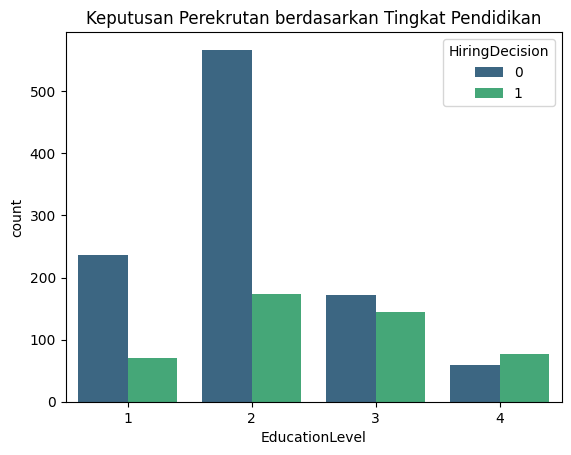
\includegraphics[width=0.6\textwidth]{gambar/barplot3.png}
    \caption{Bar Plot EducationLevel vs HiringDecision}
    \label{fig:barplot3}
\end{figure}

Dari Gambar \ref{fig:barplot3}, kita dapat melihat bahwa kandidat dengan EducationLevel yang lebih tinggi cenderung memiliki peluang lebih besar untuk diterima (HiringDecision = 1). Namun ada beberapa temuan unik, seperti kandidat dengan EducationLevel 4 (S3/PhD) memiliki peluang diterima yang lebih rendah dibandingkan dengan kandidat dengan EducationLevel 2 (S1 Tipe 2) dan 3 (S2). Hal ini menunjukkan bahwa meskipun tingkat pendidikan yang lebih tinggi umumnya dianggap sebagai keunggulan, faktor lain seperti pengalaman kerja, keterampilan, dan penilaian wawancara juga memainkan peran penting dalam keputusan perekrutan.

Untuk menjawab pertanyaan ketiga, kita dapat membuat bar plot yang menunjukan hubungan antara Gender dan HiringDecision. Gambar \ref{fig:barplot4} menunjukan bar plot dari distribusi Gender berdasarkan HiringDecision.

\begin{figure}[H]
    \centering
    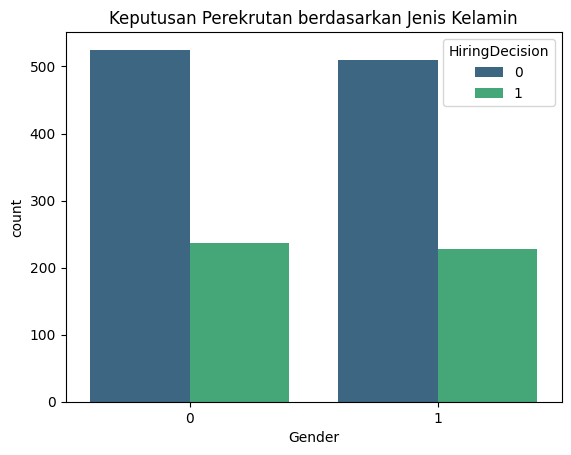
\includegraphics[width=0.6\textwidth]{gambar/barplot4.png}
    \caption{Bar Plot Gender vs HiringDecision}
    \label{fig:barplot4}
\end{figure}

Dari Gambar \ref{fig:barplot4}, kita dapat melihat bahwa kandidat Pria maupun Wanita memiliki proporsi yang seimbang baik yang diterima maupun yang tidak diterima. Hal ini menunjukkan bahwa proses perekrutan dalam dataset ini tidak menunjukkan bias yang signifikan terhadap jenis kelamin, dan keputusan perekrutan lebih dipengaruhi oleh faktor-faktor lain seperti keterampilan, pengalaman, dan penilaian wawancara.

Untuk menjawab pertanyaan keempat, kita dapat membuat bar plot yang menunjukkan hubungan antara RecruitmentStrategy dan HiringDecision. Gambar \ref{fig:barplot5} menunjukkan bar plot dari distribusi RecruitmentStrategy berdasarkan HiringDecision.

\begin{figure}[H]
    \centering
    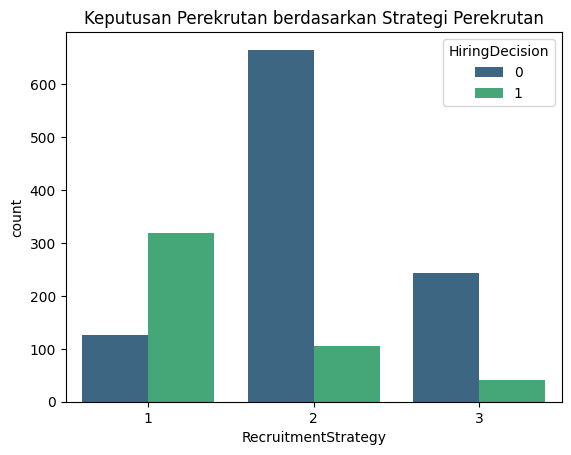
\includegraphics[width=0.6\textwidth]{gambar/barplot5.png}
    \caption{Bar Plot RecruitmentStrategy vs HiringDecision}
    \label{fig:barplot5}
\end{figure}

Dari Gambar \ref{fig:barplot5}, kita dapat melihat bahwa kandidat yang direkrut melalui strategi agresif (RecruitmentStrategy = 1) memiliki peluang lebih besar untuk diterima (HiringDecision = 1) dibandingkan dengan strategi moderat (2) dan konservatif (3). Hal ini menunjukkan bahwa strategi perekrutan yang lebih proaktif dan intensif cenderung menghasilkan kandidat yang lebih sesuai dengan kebutuhan perusahaan, sehingga meningkatkan peluang mereka untuk diterima dalam proses seleksi.

Dengan analisa yang dilakukan sebelumnya, kita sudah mengetahui bahwa beberapa fitur kategorikal memiliki korelasi yang signifikan dengan target, seperti EducationLevel dan RecruitmentStrategy. Namun uji statistik tetap perlu dilakukan untuk memastikan fitur-fitur yang akan digunakan dalam pemodelan adalah fitur yang benar-benar memiliki korelasi yang signifikan dengan target. Karena label target adalah kategorikal (1/0) dan fitur yang akan diuji juga kategorikal, maka uji statistik yang tepat adalah uji Chi-Square. Berikut adalah hasil uji Chi-Square yang dilakukan pada fitur-fitur kategorikal dalam dataset. Tabel \ref{tb:chi-square} merangkum hasil uji Chi-Square untuk setiap fitur kategorikal.

% Chi-square test for Gender: chi2 = 0.0009776541, p-value = 0.97505624092456311124976764403982087969779968261718750000000000000000000000000000000000000000000000000000000000000000000000000000000000000000000000000000000000000000000000000000000000000000000000000000
%   -> No significant association between Gender and HiringDecision (p >= 0.05)
% Chi-square test for EducationLevel: chi2 = 103.6746891896, p-value = 0.00000000000000000000025190323277589304132766103274650912631354441326531525047926129631803426889291586121544241905212402343750000000000000000000000000000000000000000000000000000000000000000000000000000
%   -> Significant association between EducationLevel and HiringDecision (p < 0.05)
% Chi-square test for RecruitmentStrategy: chi2 = 489.6813086798, p-value = 0.00000000000000000000000000000000000000000000000000000000000000000000000000000000000000000000000000000000004645739720431345829456101735102532682645682331095024667245378330315132293497743805320262196267
%   -> Significant association between RecruitmentStrategy and HiringDecision (p < 0.05)


\begin{table}[H]
    \centering
    \caption{Hasil Uji Chi-Square Fitur Kategorikal}
    \label{tb:chi-square}
    \begin{tabular}{|l|l|l|l|}
    \hline
    \rowcolor[HTML]{EFEFEF} 
    Fitur               & $Chi^{2}$    & P-Values     & Kesimpulan                     \\ \hline
    Gender              & 0.9750 & $9.75 \times 10^{-1}$ & Tidak ada perbedaan signifikan (\(p >= 0.05\)) \\ \hline
    EducationLevel      & 103.67 & $2.52 \times 10^{-22}$ & Ada perbedaan signifikan (\(p < 0.05\))       \\ \hline
    RecruitmentStrategy & 489.68 & $4.65 \times 10^{-62}$ & Ada perbedaan signifikan (\(p < 0.05\))      \\ \hline
    \end{tabular}
\end{table}

Dari tabel \ref{tb:chi-square} dapat kita lihat bahwa analisa kita sebelumnya terbukti benar terkait perbedaan signifikan, terutama pada fitur Gender yang tidak memiliki perbedaan signifikan. Sedangkan pada fitur EducationLevel dan RecruitmentStrategy terbukti memiliki perbedaan yang signifikan. Dengan demikian, fitur-fitur ini dapat dipertimbangkan untuk dimasukkan dalam model prediksi karena memiliki pengaruh yang kuat terhadap keputusan perekrutan.
\newpage
\subsection{Kesimpulan Hasil EDA}
Berdasarkan analisis data yang telah dilakukan, dapat disimpulkan beberapa hal penting terkait fitur-fitur dalam dataset dan hubungannya dengan keputusan perekrutan (HiringDecision):

\begin{enumerate}
    \item Fitur numerik seperti \texttt{InterviewScore}, \texttt{SkillScore}, dan \texttt{PersonalityScore} menunjukkan perbedaan yang signifikan antara kandidat yang diterima dan tidak diterima. Fitur-fitur ini memiliki pengaruh yang kuat terhadap keputusan perekrutan dan sebaiknya dipertimbangkan dalam pemodelan.
    \item Fitur kategorikal seperti \texttt{EducationLevel} dan \texttt{RecruitmentStrategy} juga menunjukkan perbedaan yang signifikan dengan keputusan perekrutan. Kandidat dengan tingkat pendidikan yang lebih tinggi dan yang direkrut melalui strategi agresif cenderung memiliki peluang lebih besar untuk diterima.
    \item Dari total 1500 kandidat yang ada, hanya sekitar 31\% yang diterima, menunjukkan bahwa proses perekrutan cukup selektif.
    \item Tidak ada bias signifikan terhadap Usia dan jenis kelamin dalam proses perekrutan, dengan proporsi pria dan wanita yang diterima dan tidak diterima cukup seimbang serta rentang usia yang seimbang menandakan usia dan gender bukan faktor penentu utama dalam keputusan perekrutan. Sehingga tim perekrutan dapat dikatakan profesional dan objektif dalam menilai kandidat.
    \item Fitur-fitur seperti \texttt{Age}, \texttt{PreviousCompanies}, dan \texttt{DistanceFromCompany} tidak menunjukkan perbedaan yang signifikan dengan keputusan perekrutan, sehingga mungkin kurang relevan untuk dimasukkan dalam model prediksi.
    \item Berdasarkan hasil uji statistik, fitur-fitur yang memiliki perbedaan signifikan dengan keputusan perekrutan dapat diprioritaskan dalam pemodelan untuk meningkatkan akurasi prediksi.
\end{enumerate}

Dengan demikian, fitur-fitur yang telah diidentifikasi sebagai signifikan dapat digunakan untuk membangun model prediksi yang lebih akurat dalam menentukan keputusan perekrutan di masa depan. Langkah selanjutnya adalah melakukan pemodelan menggunakan fitur-fitur tersebut dan mengevaluasi kinerja model yang dihasilkan.

\subsection{Feature Selection}
\subsection{Preprocessing}







